\documentclass{article}
\usepackage{graphicx} % new way of doing eps files
\usepackage{listings} % nice code layout
\usepackage[usenames]{color} % color
\definecolor{listinggray}{gray}{0.9}
\definecolor{graphgray}{gray}{0.7}
\definecolor{ans}{rgb}{1,0,0}
\definecolor{blue}{rgb}{0,0,1}
% \Verilog{title}{label}{file}
\newcommand{\Verilog}[3]{
  \lstset{language=Verilog}
  \lstset{backgroundcolor=\color{listinggray},rulecolor=\color{blue}}
  \lstset{linewidth=\textwidth}
  \lstset{commentstyle=\textit, stringstyle=\upshape,showspaces=false}
  \lstset{frame=tb}
  \lstinputlisting[caption={#1},label={#2}]{#3}
}

\author{Shaun Gordon and Sam Sahli}
\title{Program Counter Part Two}

\begin{document}
\maketitle

\section{Introduction}
The purpose of this lab was to create a series of test benches which would ensure the functionality of both an adder, which would be used as an incrementer for the program counter, and multiplexer, which would be used as a method of input selection.

\section{Interface}
This lab was divided into two main interests, the adder and the multiplexer.

The adder tested in this lab consisted of two register inputs, a wire output, and a register output. The two register inputs 'Ain' and 'Bin', both 32 bits, were added together and this combination was the wire output labeled 'addout'. These values Ain and Bin were manipulated across a variety of numbers to ensure full functionality, including maximum and minimum values, and a register output labeled 'Answer' was created in order to ensure the accuracy of the adder.

The mux tested in this lab consisted of three register inputs and a wire output. Two of the register inputs, labeled 'Ain' and 'Bin', were 5 bits, were used to store values. The third input labeled 'control' was used to hold a value of either 1 or 0, correlating to on and off accordingly. When the control input was off, the value stored in Ain would be displayed, and when the control was on, the displayed value would switch to Bin.  

\section{Design}
In this lab, there were two modules which were expected to be tested. The multiplexer has two inputs and a control wire and is responsible for determining which value will be sent to the program counter based on the control wire. In this sense, the multiplexer acts as a selector depending on whether the control wire is high or low.

The second module to be tested is the adder. The adder has two inputs and an output which is made up of the addition of the two inputs. By using one value as a base and the second value as a measure of incrementation, the output can be seen as an end result. This adder is used by the program counter in order to advance to the next address.

\section{Implementation}
The implementation code for the adder can be found below in Listing 1. This module is built by first including the definitions header so that word size is able to be utilized. Next the two inputs and single output are declared. The two inputs will be the numbers added together, labeled simply as Ain and Bin for simplicity, and the output will be the result of the addition labeled simply addout. All of these have been made size word because they are to hold integers of maximum 32 bit size. Because the value of addout is assigned, the output must be a wire as opposed to a register which cannot be continuously driven.

\Verilog{Verilog code for implementing an adder.}{code:add}{H:/CompOrg/ProgramCounter/Code/adder.v}

The implementation code for the multiplexer can be found below in Listin 2. This module begins by first declaring the default parameter size of 8. Because this multiplexer will be used in relation to addresses, the inputs we use will be of size 5 bits. The two inputs, Ain and Bin, are registers, along with the control wire. The output will be either the Ain value or the Bin value, depending on whether the control wire is high or low. This displayed value could be either Ain or Bin, but for our program, we decided that control low would display Ain, while control high would display Bin. 
 
\Verilog{Verilog code for implementing a multiplexer.}{code:mux}{H:/CompOrg/ProgramCounter/Code/mux.v}

\section{Test Bench Design}
The test bench for the adder is displayed in Listing~\ref{code:addtest} on page~\pageref{code:addtest}. This test bench was designed to test that the adder would indeed take in two values and output the addition of those two inputs. To proceed forward, we wanted to ensure the ability to add negative number, as well as well cycle back to zero in the case of overflow. The test bench confirms these inquiries by first adding two numbers and comparing the result with the known result labeled 'Answer'. Additionally, the test bench then takes an input of maximum value and adds to it.In reading the results of the adder, we changed the displayed values to unsigned decimal in order to better read the values of each input and output.



\Verilog{Verilog code for testing an adder.}{code:addtest}{H:/CompOrg/ProgramCounter/Code/addertester.v}

The test bench for the multiplexer is displayed in
Listing~\ref{code:muxtest} on page~\pageref{code:muxtest}. This test bench was designed to test that the mux would select Ain on control low and Bin on control high. Furthermore, it was expected that each register would have the ability to hold a maximum value of 31 which was confirmed by the test bench. In reading the results of the multiplexer, we changed the displayed values to unsigned decimal in order to better read the values of each input and output.

\Verilog{Verilog code for testing an adder.}{code:muxtest}{H:/CompOrg/ProgramCounter/Code/muxtester.v}

\section{Simulation}
The timing diagram for the adder is diplayed in Figure~\ref{fig:addtest} on page~\pageref{fig:addtest}. This diagram shows that each input can hold a minimum value of zero as well as a maximum value of 32 bits. Additionally, the diagram also confirms the adders ability to operate effectively under the expectations of the user to include negative numbers and overflow.

\begin{figure}
	\begin{center}
		\caption{Timing diagram for incrementation.}\label{fig:addtest}
		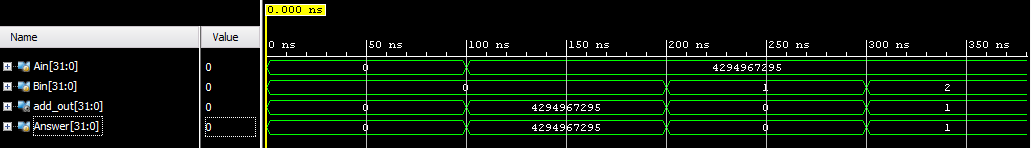
\includegraphics[width=0.9\textwidth]{H:/CompOrg/ProgramCounter/Images/ADDERTEST.png}
	\end{center}
\end{figure}

The timing diagram for the multiplexer is displayed in Figure~\ref{fig:muxtest} on page~\pageref{fig:muxtest}. This diagram shows the switching of the control wire from high to low, and the correlating display of either Ain or Bin. On control low, the Ain values are displayed to in include a maximum value of 31, and on control high, the Bin values are displayed.
 
\begin{figure}
\begin{center}
\caption{Timing diagram for value selection.}\label{fig:muxtest}
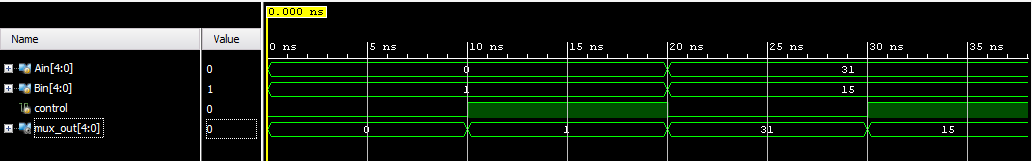
\includegraphics[width=0.9\textwidth]{H:/CompOrg/ProgramCounter/Images/MUXTEST.png}
\end{center}
\end{figure}



\section{Conclusions}
In this second lab, we sought out to create two modules with the purpose of tackling the variety of situations that a program counter may undergo. The adder would act as a means of incrementing between address values, and the multiplexer would serve as a means of input selection. In conclusion, this lab was a success with very little hinderance. One thing that was made more clear was the difference between a wire and a register and the use of each.
\end{document} 